%[Similar to reular neural networks,]\emph{Convolutional networks} [were|are] [originally] inspired by [models of] the visual cortex~\cite{Fukushima1980} but, [like|as|similar to] regular neural networks, [[they [have]] evolved to ]favor practical performance over biological accuracy.
\emph{Convolutional networks} are inspired by models of the visual cortex~\cite{Fukushima1980} but, like regular neural networks, favor practical performance over biological accuracy.
% Modern convolutional networks were [introduced|used for the first time] [in 1998] [[and [used|tested] them| demostrated their use to successfully recognize handwritten digits from the MNIST data set]~\cite{LeCun1998}.
Modern convolutional networks were introduced in 1998: LeCun et al. used them to successfully recognize handwritten digits from the MNIST data set~\cite{LeCun1998}.
Recently, Krizhevsky et al. achieved state-of-the-art performance on the ImageNet Large-Scale Visual Recognition Challenge~\cite{Krizhevsky2012}, an image classification and object localization challenge with 1000 categories~\cite{Russakovsky2015}. Thanks to recent developments, convolutional networks have become one of the most popular methods for image classification and the driving force behind deep learning.

%Classifying an image reduces, in principle, to learning the underlying function $f(x)$ that maps any image $x$ to a score vector representing the (unnormalized log probabilities of x belonging to any class.

%[To classify|Classifying] images with regular[---non-convolutional---]neural networks [requires|demands] [impractical amounts|an immesity|an enourmous amount|an abundance|lots|a good deal] of data and time [due to |because] [the size of $\Theta$| the number of learnable parameters $\Theta$ [becomes huge].]
%Due to the number of parameters that need to be learned, classifying images with regular neural networks requires impractical amounts of data and time; for instance, a small grayscale image of size $100\times100$ produces a 10\,000-dimensional input vector---10\,000 units in the input layer---, therefore, each unit in the second layer needs to learn 10\,000 parameters and a simple 2-layer neural network with 100 units in the second layer will need to learn 1\,000\,000 parameters.

Due to the number of parameters that would need to be learned, classifying images with regular neural networks is unfeasible; for instance, a small $100\times100$ grayscale image amounts to 10\,000 units in the input layer---a 10\,000-dimensional input vector---, therefore, a unit in the second layer would need to learn 10\,000 parameters and a simple two-layer network with 100 units in its second layer would have 1\,000\,000 parameters. Besides, even if data and time requirements were unrestrictive, a regular neural network would destroy the original structure of the image hindering learning. Convolutional networks take advantage of the 2-dimensional structure of images to reduce the number of parameters and facilitate learning.

Layers in a convolutional network are \emph{sparsely connected}, i.e., a unit connects only to a small subset of the units in the previous layer, and \emph{locally connected}, i.e., a unit connects to other units considering their position in the original image. Convolutional networks force \emph{weight sharing} between units in the same layer, i.e., different units share the same parameters. Lastly, \emph{pooling} subsamples the image reducing the spatial dimensions and adding invariance to local translations. All these features arise from the definition of convolutional networks, which we discuss below.

Each layer in a convolutional network is a set of \emph{feature maps}, 2-dimensional grids of unit activations ($\mathbb{R}^{h\times w}$), arranged into a 3-dimensional \emph{volume} ($\mathbb{R}^{h\times w \times d}$).
%---the third dimension joins all feature maps.~\footnote{Flattening each volume into a vector produces the equivalent neural network, although not fully-connected.}
The input layer is a volume ($\mathbb{R}^{h\times w \times c}$) that holds the input image of size $w\times h$ with $c$ color channels. The output layer is a volume of size $R^{1\times 1 \times K}$ where feature maps are single activations ($R^{1\times 1}$) representing the final score for each $k$ class. The network receives an image $x$ as an input volume that is transformed layer by layer into new volumes (whose dimensions may differ from the previous ones) until it reaches the output layer of size $h_\Theta(x) = R^{1\times 1 \times K}$(Fig.~\ref{fig:ConvNetVolumes}).

\begin{figure}[h]
	\centering
	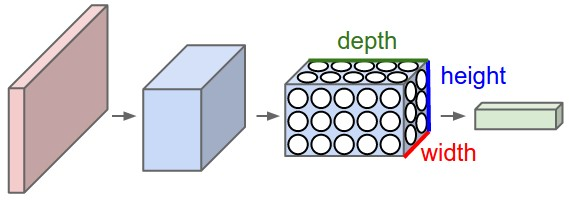
\includegraphics[width = 0.73\textwidth]{plots/convNetVolumes.jpeg}
	\caption[Illustration of a convolutional network]{Transformations computed by a convolutional network. Input layer is shown in pink, hidden layers are shown in blue and output layer is shown in green. The third layer has 5 feature maps of size $2\times3$ (width is listed first by convention). Image courtesy of~\cite{Karpathy2016}.}
	\label{fig:ConvNetVolumes}
\end{figure}

We buid a convolutional network using four types of layers: convolutional layer, ReLU layer, pooling layer and fully connected layer; all of which compute a differentiable function on its input.

\paragraph{Convolutional layer} Convolutional layers are the heart of convolutional networks. They apply filters to the volume in the previous layer; a \emph{filter} is a matrix of weights that has a small spatial size (width and height) but goes across all feature maps of the volume (the third dimension). For instance, a $3\times 3$ filter applied to a volume with 10 feature maps will have 90 parameters ($\mathbb{R}^{3\times3\times10}$) (Fig.~\ref{fig:ConvLayer}).
Feature maps are computed separately and stacked together to form the output volume of the layer. A feature map is obtained by sliding a filter across the spatial dimensions of the previous volume calculating the dot product (a weighted sum) between the filter and the input at each position~\footnote{Each filter also adds a bias term.}.
All values in a single feature map are computed using the same filter; these filters are the parameters that need to be learned.

We could think of each filter as looking for an specific feature on the input and the feature map as showing its likelihood at each position. If we regard each feature map as a grid of units, we notice that units connect only to a small local subset of units in the previous volume and that all of them share the same weights (Fig.~\ref{fig:ConvLayer}).
\begin{figure}[h]
	\centering
	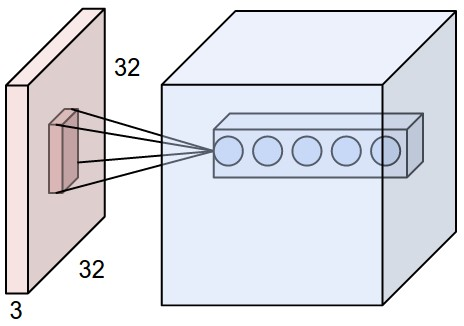
\includegraphics[width = 0.36\textwidth]{plots/convLayer.jpeg}
	\caption[Convolutional layer applied to a volume]{Convolutional layer applied to a volume ($\mathbb{R}^{32\times 32\times 3}$). The resulting volume has five feature maps as shown by the units in the blue volume ($\mathbb{R}^{32\times 32\times 5}$). Five small filters slide accross the spatial dimensions ($32\times 32$) of the volume to produce the feature maps. Image courtesy of~\cite{Karpathy2016}.}
	\label{fig:ConvLayer}
\end{figure}

We choose four hyperparameters for this layer: number of filters, filter size, stride (the number of places to shift the filter at each step) and amount of padding around the volume; these define the shape of the resulting volume. The number of filters depends on the amount of distinct features we wish to learn, the filter size is usually small ($3\times3$ to $9\times9$), stride is 1 and zero-padding is usually $\lfloor (f_s-1)/2\rfloor$ where $f_s$ is the filter size; the last one is needed to preserve the spatial dimensions of the volume in the previous layer.

\paragraph{ReLU layer} This layer performs an elementwise ReLU activation function to the volume in the previous layer, i.e., each value $z$ in the volume is passed through the nonlinearity $\max(0,z)$. It outputs a volume with the same dimensions of the previous one and has no parameters to learn. A ReLU layer (or any other activation function) usually follows a convolutional layer so it is sometimes considered part of it; we separate them for clarity. 

\paragraph{Pooling layer} The pooling layer subsamples the volume in the previous layer reducing the size of its feature maps but keeping their number. Max pooling slides a fixed-sized windows (normally $2\times2$) with stride 2 (without overlapping) along each feature map and selects the maximum element on that space. This reduces each feature map dimension by half reducing the total number of activations by 75\%, e.g., a $4\times4$ feature map gets subsampled to a $2\times 2$ feature map where values are the maximum activation in each of the four quadrants of the original feature map. Pooling is applied to each feature map separately. A popular variant of max pooling uses $3\times 3$ windows with stride 2, allowing for overlapping.

\paragraph{Fully connected layer} A fully connected layer is a convolutional layer with $w\times h$ filters where $w$ and $h$ are the spatial dimensions of the volume in the previous layer and no zero-padding, i.e., filters cover the entire volume, resulting in feature maps with size $1 \times 1$. The output layer of a convolutional network is always fully connected with as many feature maps as possible classes.% We interpret the scores of the output layer like those of regular neural networks as the (unnormalized log) probability of $x$ belonging to class $k$.  

\bigskip
%[The reasoning behind is] Convolutional layers (plus ReLU layers) compute features on the input while pooling layers shrinken the volume before passing to the fully connected layers that act as a regular neural network classifier on the obtained features.

The standard convolutional network architecture can be represented textually as:
\begin{verbatim}
INPUT -> [[CONV -> RELU]*N -> POOL?]*M -> [FC -> RELU]*K -> FC
\end{verbatim}
where \texttt{*N} indicates that the components are repeated \texttt{N} times, \texttt{?} indicates an optional component and \texttt{N,M,K >= 0}. We use this template to build a large range of models from a linear classifier \texttt{INPUT -> FC} (\texttt{N,M,K = 0}) to a regular neural network \texttt{INPUT -> [FC -> RELU]+ -> FC} (\texttt{N,M = 0}, \texttt{K > 0}) to a convolutional network \texttt{INPUT -> [[CONV -> RELU]+ -> POOL?]+ -> [FC -> RELU]* -> FC} (\texttt{N,M > 0}, \texttt{K >= 0}).

For example, a typical deep convolutional network could be:
\begin{verbatim}
INPUT -> [[CONV -> RELU]*2 -> POOL]*3 -> [FC -> RELU]*2 -> FC
\end{verbatim}
This network receives an input volume (the image), computes two sets of convolution plus ReLUs before pooling and repeats this pattern three times followed by fully connected layers plus ReLUs which are repeated twice and the output layer that reports the final classification scores. Although there is not a standard way of counting the number of layers, we usually ignore ReLU and pooling layers because they lack learnable parameters. Therefore, our network has 10 layers (21 in total), which is a good depth for big data sets. Practical advice on choosing an architecture is offered in Section~\ref{sec:PracticalDL}.

Figure~\ref{fig:ConvNetExample} shows a convolutional network with different kinds of layers. The image was obtained in a simulation accesible at \url{cs231n.stanford.edu}.

\begin{figure}[h]
	\centering
	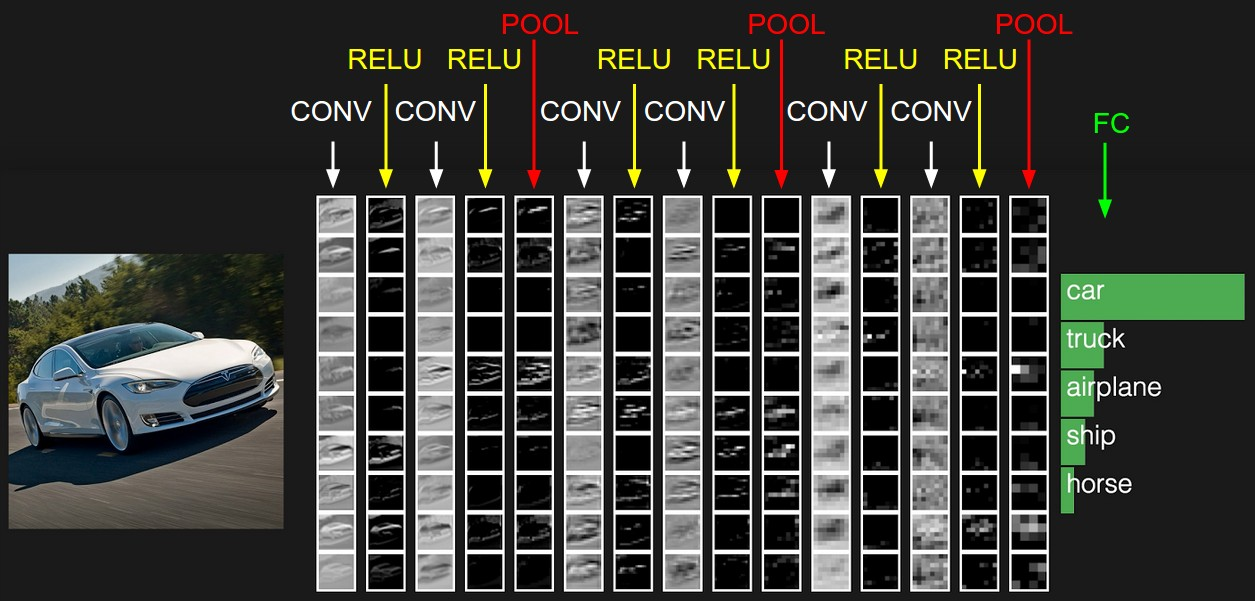
\includegraphics[width = 0.92\textwidth]{plots/convNetExample.jpeg}
	\caption[Convolutional network in action]{Convolutional network with architecture \texttt{INPUT -> [[CONV -> RELU]*2 -> POOL]*3 -> FC}. The input image has size $32\times 32$. Each hidden layer (a column) has 10 feature maps. Although the size of feature maps looks constant, each pooling layer reduces its dimensions by half (after the final pooling layer, feature maps have size $4\times 4$). We show final scores for the five most probable classes. Image courtesy of~\cite{Karpathy2016}.}
	\label{fig:ConvNetExample}
\end{figure}

Lately, simpler convolutional network architectures have emerged. The All Convolutional Net~\cite{Springenberg2014} is a network formed solely by convolutional layers: we replace pooling layers with convolutional layers with the same number of filters, filter size and stride; it learns the pooling operation.
% This greatly increases the number of parameters so it is inappropiate for small data sets.
\emph{Transfer learning} is a related trend where we train a convolutional network on data from a specific domain and later reuse it to extract image features in a different domain or as an initial network to fine-tune with new data.

The loss function for a multiclass convolutional network is similar to that for a regular neural network (Eq.~\ref{eq:ANNRegularizedLossFunction}) except that, in this case, the convolutional network defines the vector score $h_\Theta(x)$.
\begin{equation}
	L(\Theta) = -\frac{1}{m} \sum_{i=1}^m \log \left ( \frac{ e^{h_\Theta(x^{(i)})_{y^{(i)}}} }{ \sum_{j=1}^K e^{ h_\Theta (x^{(i)})_j} } \right ) + \frac{\lambda}{2m}\sum_{l=1}^{L-1}\sum_{i=1}^{s^{(l)}}\sum_{j=1}^{s^{(l+1)}} \left(\Theta^{(l)}_{ij}\right)^2
	\label{eq:ConvNetLossFunction}
\end{equation}
This function is differentiable with respect to $\Theta$, thus, we can train the entire network via gradient descent. We calculate the gradient of the loss function with backpropagation.% We use backpropagation to calculate the gradient of the loss function.

\begin{comment}
In this section we revised the standard features and training of current convolutional networks. For an in depth review of convolutional networks, see \cite{Karpathy2016}. For a complete overview of the history and state of deep learning, see \cite{Schmidhuber2015}. Section~\ref{sec:PracticalDL} gives some practical advice for choosing hyperparameters and training deep architectures.
\end{comment}
